Por se tratar de um ambiente de simulação de realidade virtual, alguns parâmetros foram identificados a fim de estabelecer a melhor relação física entre o dispositivo projetado e a verdadeira sensação de um passeio ou corrida de bicicleta. Os sistemas foram desenvolvidos de acordo com os requisitos estabelecidos pelo projeto e posteriormente integrados entre as frentes de controle, estrutura e software presentes no mesmo.

\section{Sistema de Elevação Vertical Dianteiro}

Em um simples passeio de bicicleta é comum lidarmos com situações adversas de terreno, ou seja, variações na declividade em razão a existência de subidas e descidas bem como ainda a existência de planos. O V-Ride conta com um sistema de acionamento vertical dianteiro que emula a realidade entendida pelo usuário quando imerso em ambiente de variações de terreno significativas. 
O acionamento figura-se em um princípio básico de ativação: um motor acoplado a um eixo presente em um macaco hidráulico movimenta um parafuso de potência transformando o movimento horizontal linear em movimento vertical linear. Todo princípio de acionamento é controlado pela atuação de um motor, sendo assim, a escolha do mesmo é fundamental para a determinação do correto movimento a ser transmitido, e por conseqüência garantir a movimentação dianteira em concordância a simulação de realidade pretendida. 
Por se tratar de um movimento de caráter sensível e preciso, o projeto V-Ride encontrou na modernidade a facilidade no emprego de uma tecnologia consolidada no mercado: o macaco elétrico. A tecnologia viabiliza a operação funcional do sistema de elevação vertical, uma vez que quando  dimensionado,o torque, executado pelo motor é capaz de saciar as necessidade de carga exigidas pelo usuário.

\subsection{Motor Elétrico}

O motor elétrico é um dispositivo que converte energia elétrica em energia mecânica. O mesmo pode ser operado mediante alimentação de corrente contínua ou alternada. O princípio de funcionamento de um motor elétrico se dá pela interação entre campos eletromagnéticos. A existência de uma força mecânica gerada por uma corrente que flui sobre um fio nele presente, quando imerso em um campo magnético, viabiliza e rotação de uma de suas partes, o rotor. 
                 
                        \begin{center}
    	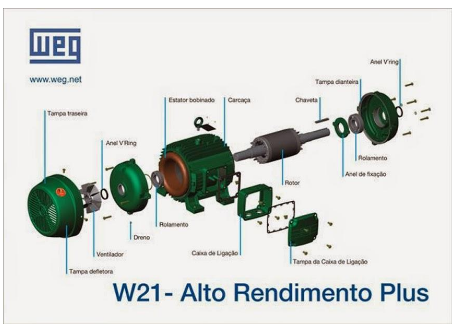
\includegraphics[scale=0.7]{figuras/rotor}
        \captionof{figure}{Componentes de um motor elétrico. Fonte:  Zona da Tecnologia}
        \label{rotor}
    \end{center}


Principais componentes de um motor elétrico: 
     \begin{itemize}
    \item 
     I . Rotor
         \item 
 O rotor é o componente que gira em uma máquina elétrica. Ele é formado por um eixo que abriga um conjunto de bobinas enroladas sobre um núcleo magnético que pode girar sobre um campo magnético criado por um imã ou um conjunto de bobinas presentes no estator.
 \item 

  II. Estator 
 \item 
O estator é a parte fixa do motor e tem por finalidade conduzir o fluxo magnético para rotação do rotor, parte móvel da máquina elétrica. É no estator que é criado um campo magnético capaz de induzir corrente elétrica no conjunto móvel.

    \end{itemize}

     
\subsection{Dimensionamento}

Antes de qualquer aplicação prática, um dimensionamento prévio deve ser estabelecido a fim de determinar a escolha do melhor motor para uso. Com isso, um estudo prévio deve ser feito a fim de garantir a funcionalidade e aplicabilidade pretendidas com o uso da máquina elétrica. Alguns parâmetros foram então identificados e determinados como forma de garantir o correto dimensionamento do motor. 
 \item 
- Análise das forças envolvidas: 
 \item 
                                  
                            
 \begin{center}
    	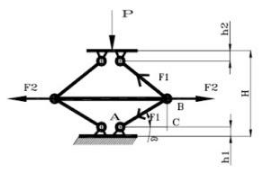
\includegraphics[scale=0.7]{figuras/item}
        \captionof{figure}{Diagrama de corpo livre do macaco hidráulico}
        \label{item}
    \end{center}

O valor do ângulo β presente na figura foi obtido previamente com valor aproximado de 20°. Aplicando o somatório de forças atuante sobre o braço superior direito, temos:
              \begin{center}
    	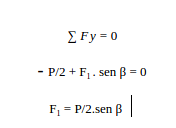
\includegraphics[scale=0.7]{figuras/f1}
                \label{f1}
    \end{center}

Considerando que o usuário, bicicleta e a mesa giratória presente na parte dianteira possuem peso aproximado de 1300 N, temos: 

          F1 = 1900,47 N       (1) 

Para a determinação de aplicação sobre o fuso do macaco, aplicamos o somatório das forças no eixo x, então: 

                       \begin{center}
    	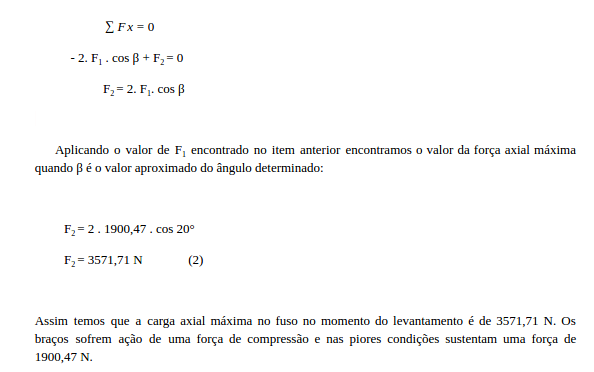
\includegraphics[scale=0.7]{figuras/f2}
                \label{f2}
    \end{center}
 \item 
- Velocidade máxima desempenhada pelo motor: 
 \item 
 A partir das especificações técnicas do motor presente no macaco elétrico, o cálculo da velocidade máxima de levantamento para a carga nominal foi calculado: 
 


 \begin{center}
      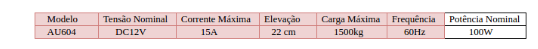
\includegraphics[scale=0.7]{figuras/calculado}
        \captionof{figure}{ Tabela 1. Especificações técnicas do motor elétrico}
        \label{calculado}
    \end{center}   
                       
    \begin{center}
      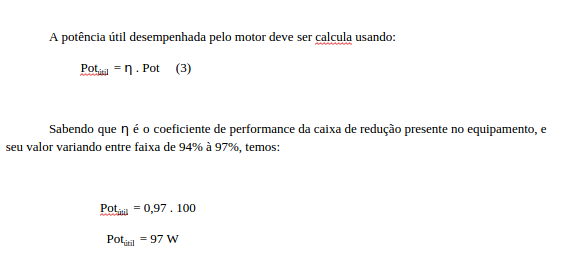
\includegraphics[scale=0.7]{figuras/f3}
                \label{f3}
    \end{center}                    

Potência mecânica é definida pela equação 4 abaixo, onde v é a velocidade desempenhada pelo motor no levantamento:  

                         
    \begin{center}
      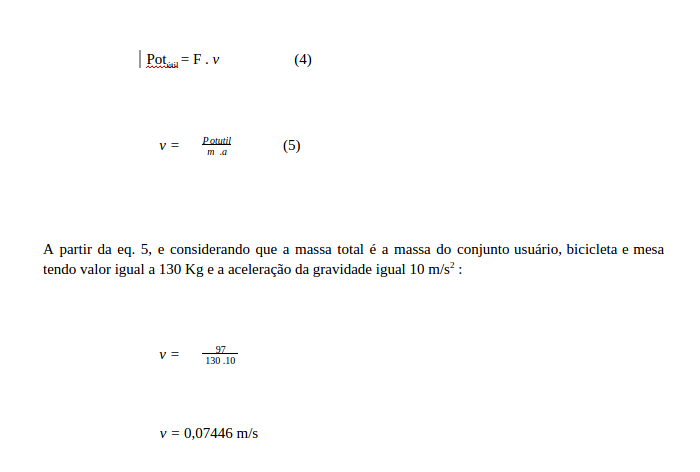
\includegraphics[scale=0.7]{figuras/f4}
                \label{f4}
    \end{center}
           
    \begin{center}
      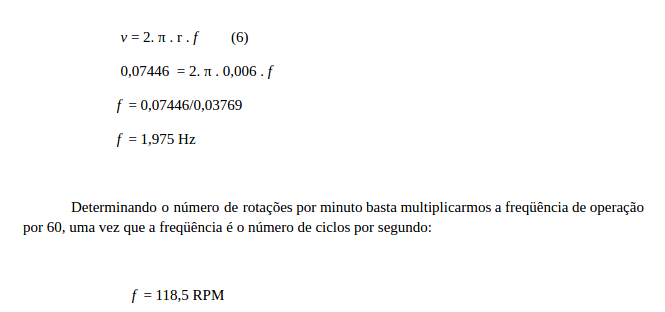
\includegraphics[scale=0.7]{figuras/f5}
                \label{f5}
    \end{center}

Dessa forma, o motor produz aproximadamente 119 rotações por minuto quando operado em velocidade nominal para a carga total associada. Esse parâmetro é variável, uma vez que a carga total é função do usuário e do peso da bicicleta acoplada no sistema. 
    \section{Sistema de Alimentação de Energia }

O conceito de sustentabilidade está cada vez mais imerso no dia a dia do ser humano. A ideia de tornar sustentável e a capacidade de reutilização tornam-se obséquio da capacidade humana em desenvolver maneiras ainda mais versáteis e inovadoras em detrimento à dependência por tecnologias já consolidadas e de alto custo de manutenção. Com isso, o projeto V-Ride conta com um sistema próprio de geração de energia elétrica a partir do movimento mecânico gerado pelas pedaladas do usuário. 
O circuito consiste em um sistema misto de alimentação. Uma fonte geradora, dínamo, e o uso da rede elétrica a fim de manter a carga sempre armazenada na bateria. 
    \subsection{Circuito carregador rede elétrica}  
O circuito integrado ao circuito gerador tem por fonte a rede elétrica residencial. Sabendo que a tensão da bateria utilizada para armazenamento da energia elétrica apresenta tensão inferior a tensão fornecida pela rede, foi necessário a construção de um carregador que atendesse aos parâmetros de carregamento da bateria. 
O dispositivo capaz de interagir com os valores disponibilizados pela rede é o transformador. Assim, o grupo adequou-se ao uso do componente que é capaz de receber uma alta tensão, oriunda da rede elétrica, e disponibilizasse a tensão de recarga indicada pelo fabricante da bateria. Por se tratar de fontes de natureza distintas, ou seja, a rede elétrica disponibiliza corrente alternada e a bateria é alimentada por corrente contínua, criou-se a necessidade de retificação da corrente de saída do transformador. A ponte retificadora consiste em configuração de diodos em ponte, ou ponte de “Wheatstone”, capaz de ‘linearizar’ o sinal oscilatório de natureza alternada. 
                                
            
 \begin{center}
    	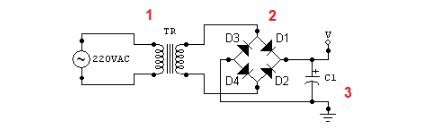
\includegraphics[scale=0.7]{figuras/alternada}
        \captionof{figure}{Esboço simplificado carregador de bateria. Fonte: Ebah}
        \label{alternada}
    \end{center}

Em 1 é possível identificarmos a presença do transformador. No primário, a tensão de entrada é de 220V, referente a rede; no secundário saída de 15V. A corrente de operação na saída do transformador é de 3A. A ponte retificadora é indicada em 2, nela o sinal entra alternado e tem saída contínuo. Em 3 é possível identificar a presença de um capacitor, o mesmo é responsável pela filtração do sinal de saída da ponte retificadora, uma vez que a retificação é de onda completa. A necessidade de incremento do banco de capacitores ao circuito se da uni e exclusivamente em razão a otimização e qualidade da corrente que será disponibilizada a bateria. 
                                                   
                               \begin{center}
    	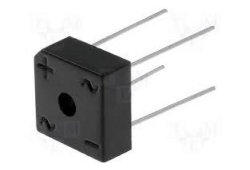
\includegraphics[scale=0.7]{figuras/bateria}
        \captionof{figure}{Ponte retificadora 10A.Fonte: Proesi}
        \label{bateria}
    \end{center}
                                             
 \begin{center}
    	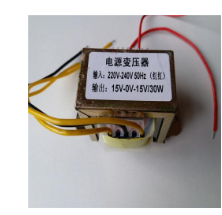
\includegraphics[scale=0.7]{figuras/trafo}
        \captionof{figure}{Transformador 220V/15V. Fonte: AliExpressi}
        \label{trafo}
    \end{center}
                            
                                        
                            \begin{center}
    	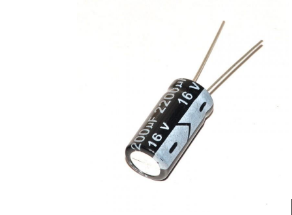
\includegraphics[scale=0.7]{figuras/capacitor}
        \captionof{figure}{Capacitor 2200µF. Fonte: Bau da Eletronica}
        \label{capacitor}
    \end{center}

  
A montagem do circuito carregador foi feito segundo a figura 8. Nela é possível identificarmos a presença de alguns componentes extra, são eles: botão liga-desliga, o porta fusível como item de segurança  e um led indicador de abertura ou fechamento do circuito. 

          
      \begin{center}
    	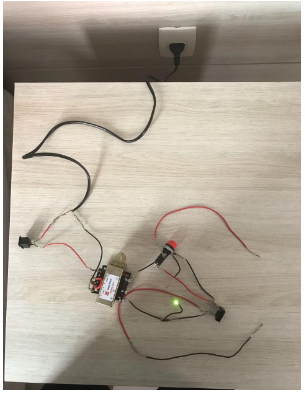
\includegraphics[scale=0.7]{figuras/circuito}
        \captionof{figure}{ Representação esquemático circuito carregadora}
        \label{circuito}
    \end{center}
A figura 11 representa a simulação por software do circuito carregador. Nela é possível analisarmos uma tensão de 15,9V na saída do transformador. A margem é aceitável, uma vez que é superior à tensão da bateria, mas não é o valor ideal, visto que o fabricante determina os valores ótimos para recarga.
   
                         
 \begin{center}
    	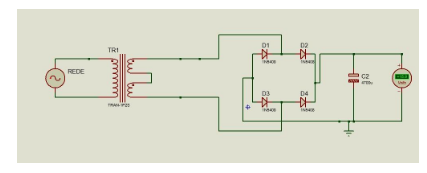
\includegraphics[scale=0.7]{figuras/esquema}
        \captionof{figure}{ Simulação do circuito do carregador }
        \label{esquema}
    \end{center}
    \section{Bateria}  
A presença de uma bateria no projeto é justificada pela necessidade de armazenamento da energia elétrica produzida. Uma vez que o projeto conta com um sistema de geração de energia, o dínamo elétrico, a energia ali produzida deve ser armazenada a fim de manter as condições de funcionamento de outros equipamentos presentes no projeto, como por exemplo os motores que atuam nos sistemas de elevação e de frenagem. 
 Para o projeto V-Ride criou-se então a necessidade do uso de uma bateria que atendesse a simples sistemas de potência, como a operação de motores. Assim, por ser alimentada por um circuito integrado que consiste em uma fonte geradora e uso da rede elétrica residencial, o primeiro passo consiste em escolher uma bateria que apresente tensão inferior a suas formas de alimentação. O passo seguinte é adequar o fornecimento de corrente elétrica necessária a correta alimentação das cargas envolvidas. A figura 4 ilustra a bateria utilizada no projeto.
                                        
                         
 \begin{center}
    	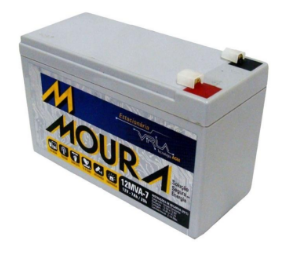
\includegraphics[scale=0.7]{figuras/projeto}
        \captionof{figure}{ Bateria Moura 12MVA-7 . Fonte: Mercado Livre }
        \label{projeto}
    \end{center}
      
Analisando todos os tipos de bateria existentes no mercado e as necessidades geradas pelos equipamentos consumidores de potência elétrica, determinou-se o uso da bateria cuja especificações estão listadas na tabela 2 abaixo.

 \begin{center}
    	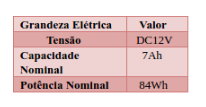
\includegraphics[scale=0.7]{figuras/tabela}
        \captionof{figure}{ Bateria Moura 12MVA-7 . Fonte: Mercado Livre }
        \label{tabela}
    \end{center}
Os valores apresentados pela tabela 2 são específicos ao tipo de bateria usado no projeto V-Ride. Podemos observar que a mesma possui uma autonomia fixa de 84Wh, ou seja, é capaz de fornecer uma potência constante de 84W por um período fixo de uma hora, suficiente e necessário para alimentação dos componentes elétricos presentes.
A figura a seguir ilustra ainda alguns parâmetros de suma importância para a correta adequação da bateria ao seu sistema de carga. 
                                           
                            
 \begin{center}
    	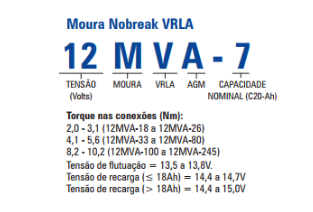
\includegraphics[scale=0.7]{figuras/esp}
        \captionof{figure}{ Especificações técnicas bateria.  Fonte: Moura  }
        \label{esp}
    \end{center}
Observamos que a mesma apresenta tensão de recarga entre os valores 14,4 V e 14,7 V, ou seja, por apresentar um sistema de alimentação misto foi necessário adequação dos sistemas de recarga ao uso de um regulador de tensão capaz de manter a tensão nos terminais de entrada da bateria dentro dos valores determinados pelo fabricante. 

    \section{Sistema de frenagem }  
 A fim de garantir as melhores condições de simulação da realidade proposta ao usuário, o V-Ride conta com um sistema que emula as condições de terreno impostas. Ou seja, em ambientes de aclividade, a sensação de um pedalar mais difícil é sentida. Tal impressão só é sentida devido a existência de um sistema sensível capaz de operar nas condições de realidade proposta.
Para isso, o acionamento é feito mediante atuação de um motor que acoplado a uma haste de ferro tracionada viabiliza o contato por atrito com uma polia presente no eixo do rolo da estrutura traseira. Por se tratar de um movimento muito preciso e sensível, a transmissão do movimento do motor para a haste deve ocorrer de maneira controlada e gradual, uma vez que o espaço percorrido até o contato é pequeno. O motor que melhor atende as condições necessárias é o motor de passo, capaz de trabalhar com pequenas variações dentro de um passo ou ainda micro passo. 

  \subsection{Motor de Passo }  
          O motor de passo é um motor elétrico usado em situações onde se deseja obter um posicionamento preciso ou ainda o rotacionamento de um ângulo exato. A rotação desenvolvida pelo motor é controlada por uma série de campos magnéticos emitidos eletronicamente por pulsos ou passos. Por não usar escovas ou comutadores, o motor possui um número fixo de pólos magnéticos que determinam o número de passos por revolução executada.  O número de passos realizados executa a variação de um certo ângulo rotacionado pelo eixo do motor, sendo o controle desses passos realizado de maneira computacional e uma das formas mais versáteis de sistema de posicionamento. 
    \subsection{Especificações do Motor de Passo }  
 O motor de passo utilizado no sistema de frenagem apresenta as especifiações listadas segundo a figura 9 abaixo: 
                                       
                            
 \begin{center}
    	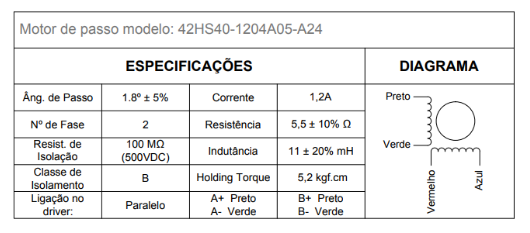
\includegraphics[scale=0.7]{figuras/tec}
        \captionof{figure}{ Dados técnicos motor de passo   }
        \label{tec}
    \end{center}
O torque de manutenção apresentado é de 5,2kgf .cm .Para as necessidades criadas o valor é superior, entretanto por ser uma máquina que estava disponível para uso apenas houve a adequação da mesma ao funcionamento do sistema de frenagem. 
Outro parâmetro considerável para análise de dimensionamento do motor é a faixa de freqüência de operação e o torque por ele produzido. Tendo em vista que o mesmo irá operar dentro de um curto período de tempo, o mesmo é capaz de satisfazer os valores entendidos para carga durante ambientes de inclinação.
                                    

 \begin{center}
    	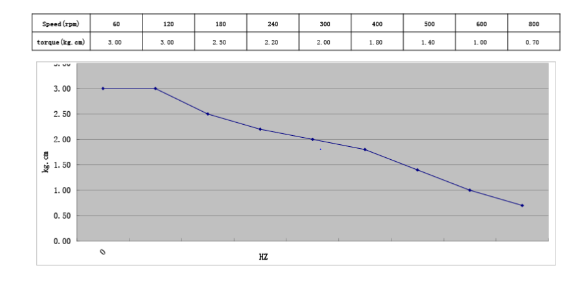
\includegraphics[scale=0.7]{figuras/torque}
        \captionof{figure}{ Curva Torque x Frequência de operação}
        \label{toque}
    \end{center}
  \subsection{Geração de Energia }  

Uma máquina elétrica nada mais é que um dispositivo que realiza a conversão entre energia mecânica e energia elétrica, quando esta conversão é feita no sentido da transformação da energia mecânica em energia elétrica esta máquina recebe o nome de gerador, esta conversão normalmente ocorre devido a atuação de um campo magnético (CHAPMAN, 2013). 

Para o escopo deste trabalho decidiu-se utilizar um alternador com o objetivo de converter a energia mecânica oriunda das pedaladas do usuário na bicicleta em energia elétrica para alimentar os componentes da solução.

As duas principais partes das máquinas elétricas são o estator e o rotor, o estator consiste em um conjunto de órgãos ligados rigidamente à carcaça, que possui bobinas com enrolamentos e o rotor é sistema rígido que gira em torno de um eixo apoiado em mancais fixos na carcaça, que é constituído por por dois núcleos polares (polos magnéticos Norte e Sul),  uma bobina indutora, dois anéis coletores e um veio. (NETTO, 2010). 

Sendo assim, podemos destacar ainda que nestas máquinas teremos um indutor que será responsável por produzir o campo magnético, e o induzido que receberá a corrente induzida, então no alternador o rotor faz o papel de indutor, enquanto o estator fará o papel de induzido, assim como a conversão obedecerá o princípio da Lei de Lenz, pois uma corrente induzida produzirá um campo magnético que por sua vez exercerá forças contrárias a rotação do rotor, isto explica a necessidade do rotor nestas máquinas elétricas demandarem acionamento mecânico (NETTO, 2010). 

Inicialmente decidiu-se por utilizar um alternador automotivo, uma vez que o mesmo atendia os requisitos de aplicação impostos pelo projeto e já possuía integrado os sistemas de retificação, regulação de tensão e proteção contra correntes reversas, as principais partes do alternador automotivo são descritos a seguir:

 \begin{center}
    	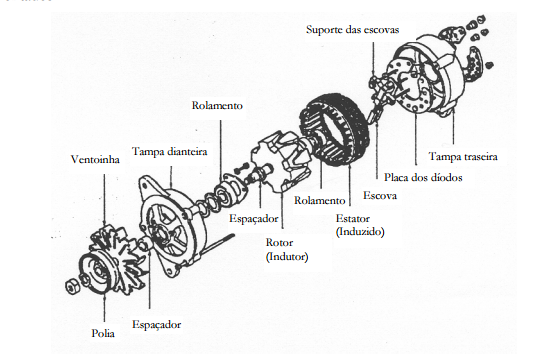
\includegraphics[scale=0.7]{figuras/partes}
        \captionof{figure}{  Partes de um Alternador. Fonte: General Motors}
        \label{partes}
    \end{center}


Como posse das supracitadas informações foi decidido por utilizar um Alternador da marca Bosh 14 V 80 A/h que foi acoplado ao rolo de treino da estrutura por uma correia que liga a polia do alternador a uma polia que foi instalada no rolo, da seguinte forma:



 \begin{center}
    	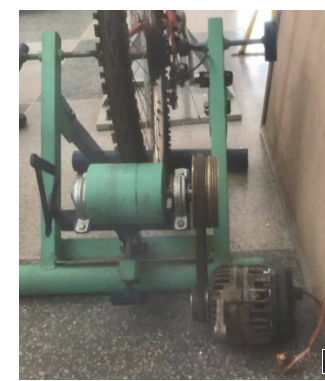
\includegraphics[scale=0.7]{figuras/alt}
        \captionof{figure}{  Alternador acoplado ao rolo de treino.}
        \label{alt}
    \end{center}

O esquema mostrado acima foi acoplado a uma bateria para serem realizados os testes de validação da solução, com o auxílio de um multímetro foi medida a corrente entre o sistema alternador/bateria. 

O alternador escolhido tem a especificação de mínima rotação para acioná-lo, sendo esta em torno de 800 RPM, no esquema montado têm-se que a relação da roda para da bicicleta para o rolo é de 6:1 e da polia do rolo para a polia do alternador de 2:1, assim sendo estipulou-se que a rotação mínima para acionar a geração de energia é de 67 RPM, o que é um valor razoável que até um usuário sedentário poderia atingir. 

Porém verificou-se experimentalmente que para as condições previstas teoricamente o alternador não era capaz de carregar a bateria uma vez que a corrente obtida na medição era negativa, ou seja o alternador não só não stava cumpindo sua função de carregar a bateria como estava puxando energia da mesma, através de revisão bibliográfica explica-se este fato devido aos componentes citados anteriormente que poderiam vir a demandar energia, assim sendo foram realizados testes em períodos maiores de tempo e variando o sistema de marchas da bicicleta. 

Averigou-se então que em marchas mais pesadas a corrente medida passava a ser positiva e aumentava gradualmente com o aumento da velocidade das pedaladas, porém a solução foi invalidada uma vez que um dos escopos do projeto é propor uma solução modular independente da bicicleta, o que não seria possível devido a dependência da marcha, foram levantadas soluções alternativas, como o aumento da relação entre as polias para causar um efeito multiplicador, porém isto causaria o mesmo efeito do aumento da marcha, ou seja o aumento da sensação de peso pelo usuário, assim sendo, só seria possível gerar energia em um sistema com marcha pesada o que inviabilizaria a simulação de cenários de descida, que é um dos propósitos do jogo. 

Como a utilização do alternador não era mais uma solução viável optou-se por utilizar dínamos de bicicleta, que possuem capacidade de produção de energia bem menos significativas, porém são adaptáveis a todos os requisitos do projeto, além de um sistema com um circuito complementar que permitirá carregar a bateria com o sistema convencional de energia elétrica oriunda da rede para suprir as possíveis demandas que o dínamo não é capaz de atender.

O dínamo que será utilizado é o seguinte:


 \begin{center}
    	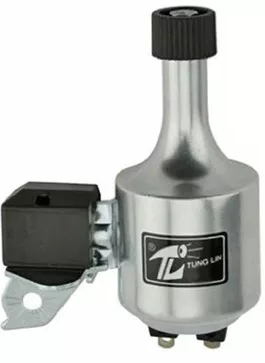
\includegraphics[scale=0.7]{figuras/dinamo}
        \captionof{figure}{  Dínamo a ser usado.}
        \label{dinamo}
    \end{center}
O critério para a seleção do mesmo foi a necessidade que o mesmo possuíssem uma tensão maior que a da bateria (12V), assim sendo, o único modelo comercial que possuía estas especificações é o da figura que possui tensão de 16 V e potência máxima de 8 W, como sabe-se que esta potência depende das rotações oriundas da pedaladas vê-se que esta é uma solução proposta apenas para aproveitar a energia mecânica que está sendo gerada. Optou-se ainda por utilizar 2 dínamos deste tipo a fim de aumentar a potência gerada sem criar complicações estruturais.  

Como a bateria tem a especificação de 7 Ah e cada dínamo libera no máximo 0.5 A, utilizando uma rotação alta a geração máxima seria 1 de Ah, logo seriam demandadas 7 horas pra carregar completamente a bateria, um tempo considerado alto, porém como os atuadores são acionados apenas esporadicamente e a geração é contínua, este tempo não é o tempo real de carga da bateria uma vez que o tempo de geração é bem maior que o tempo que energia é demandada pelos atuadores, na próxima etapa do projeto com a integração da exatidão do tempo nos cenários do jogo será possível determinar este dado com precisão.

A saída do dínamo é em formas de pulsos, ou seja demanda retificação para conectá-la a bateria que demanda corrente contínua, para tanto será utilizado um circuito retificador como o seguinte: 



 \begin{center}
    	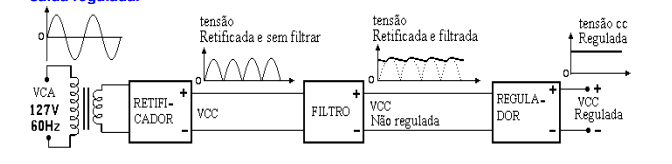
\includegraphics[scale=0.7]{figuras/ret}
        \captionof{figure}{Circuito a ser implementado em conjunto com o dínamo.}
        \label{ret}
    \end{center}

A primeira parte da retificação ocorre por meio de uma ponte de diodos em H, os diodos inicialmente usados para teste foram o 1N4004, para a filtragem é utilizado um capacitor de 4700uF que será responsável por diminuir esta pulsação, porém como visto na imagem acima a onda ainda não é completamente linear, então ocorre a estabilização através de um diodo Zenner que ainda terá a função de evitar correntes reversas que poderiam a vir da bateria para os dínamos. 






























